\documentclass[a4paper,10pt]{article}
\usepackage[english]{babel}
\usepackage{listings}
\usepackage{graphicx}

% Javascript definition
% Source: http://tex.stackexchange.com/questions/89574/language-option-supported-in-listings
\usepackage{color}
\definecolor{lightgray}{rgb}{.9,.9,.9}
\definecolor{darkgray}{rgb}{.4,.4,.4}
\definecolor{purple}{rgb}{0.65, 0.12, 0.82}
\lstdefinelanguage{JavaScript}{
  keywords={break, case, catch, continue, debugger, default, delete, do, else, false, finally, for, function, if, in, instanceof, new, null, return, switch, this, throw, true, try, typeof, var, void, while, with},
  morecomment=[l]{//},
  morecomment=[s]{/*}{*/},
  morestring=[b]',
  morestring=[b]",
  ndkeywords={class, export, boolean, throw, implements, import, this},
  keywordstyle=\color{blue}\bfseries,
  ndkeywordstyle=\color{darkgray}\bfseries,
  identifierstyle=\color{black},
  commentstyle=\color{purple}\ttfamily,
  stringstyle=\color{red}\ttfamily,
  sensitive=true
}

\lstset{
   language=JavaScript,
   backgroundcolor=\color{lightgray},
   extendedchars=true,
   basicstyle=\footnotesize\ttfamily,
   showstringspaces=false,
   showspaces=false,
   numbers=left,
   numberstyle=\footnotesize,
   numbersep=9pt,
   tabsize=2,
   breaklines=true,
   showtabs=false,
   captionpos=b
}
% end Javascript definition


\lstset {
	basicstyle=\footnotesize,
}
\title{Visualizing Spatial Data in DotA2}


\author{Koray Yanik\\ Delft University of Technology \and Haji Akhundov\\ Delft University of Technology}
        
\begin{document}
\maketitle

\section{Heatmap}
One of the most easily created and useful spatial data visualizations is a \emph{heatmap}. In our DotA2 dataset we have several matches worth of player coordinates over time. Even more interesting, we have matches from several tier brackets. Once we have a heatmap of all data, it would also be interesting to create a heatmap per tier, to compare the overall map usage per tier. After that several filters were applied to these heatmaps.

When we tried to parse the dataset in the D3 library we encountered a severe problem however: this library is not suited for datasets of this scale. To solve this issue we chose to preprocess our dataset, transforming it into a heatmap dataset usable in D3 using a different platform first. Our second step was to filter only a certain tier in this transformation. The third step was applying several visual filters to these heatmaps.

\subsection{Preprocessing [TODO]}
TODO

\subsection{Filtering [TODO]}
TODO

\subsection{Rendering the heatmap in D3}
Since our heatmap dataset consisted of a csv with for every point a triple of the following format: $(x, y, v)$ where x and y encoded the location of this point, and v the count of this position being entered in the dataset by a player, loading the heatmap in D3 was trivial.

\begin{lstlisting}[language=JavaScript]
// Maps raw map coordinates into normalized map coordinates for our screen
var xS = function (var rx);
var yS = function (var ry);
// Converts a raw value into a normalized heatmap color
var color = function (var value);
// Use the d3 CSV viewer on our heatmap dataset, load in data
d3.csv("data/HM_"+tier+"_"+filter+".csv", function (error, data) {
	// Convert every value (loaded as string) into integers
	data.forEach(function(d){
	    d.x = parseInt(d.x);
	    d.y = parseInt(d.y);
	    d.v = parseInt(d.v);
	});
	// For every point, add a rectangle to our SVG element
	dataset = container.selectAll("rect")
	    .data(data)
	    .enter()
	    .append("rect")
	    .attr("x", function (d) { return xS(d.x)})
	    .attr("y", function (d) { return yS(d.y)})
	    .attr("width",   6 ) 
	    .attr("height",  6 )
	    .style("fill",   function (d) { return color(d.v) });
});
\end{lstlisting}

\section{Zone Map}



\section{Match Replaying}

\subsection{Preproccessing and Filtering}

\subsection{Displaying Replays in D3}

\subsection{A Quicker Implementation in plain JavaScript}

\section{Conclusions}

Here we present some conclusions drawn from our visualisations.

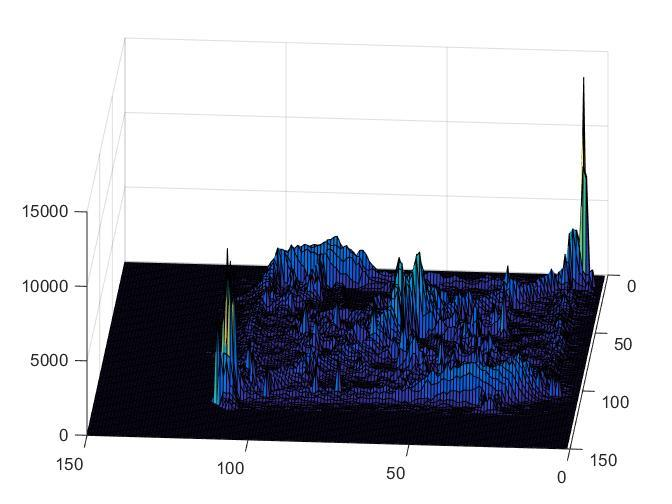
\includegraphics[width=\textwidth]{HM3D}
Here we show a raw, unnormalized 3D heatmap generated in MatLab. It shows two spikes on the starting areas. These might be the player starting positions, but almost look like outliners and might also indicate some errors.

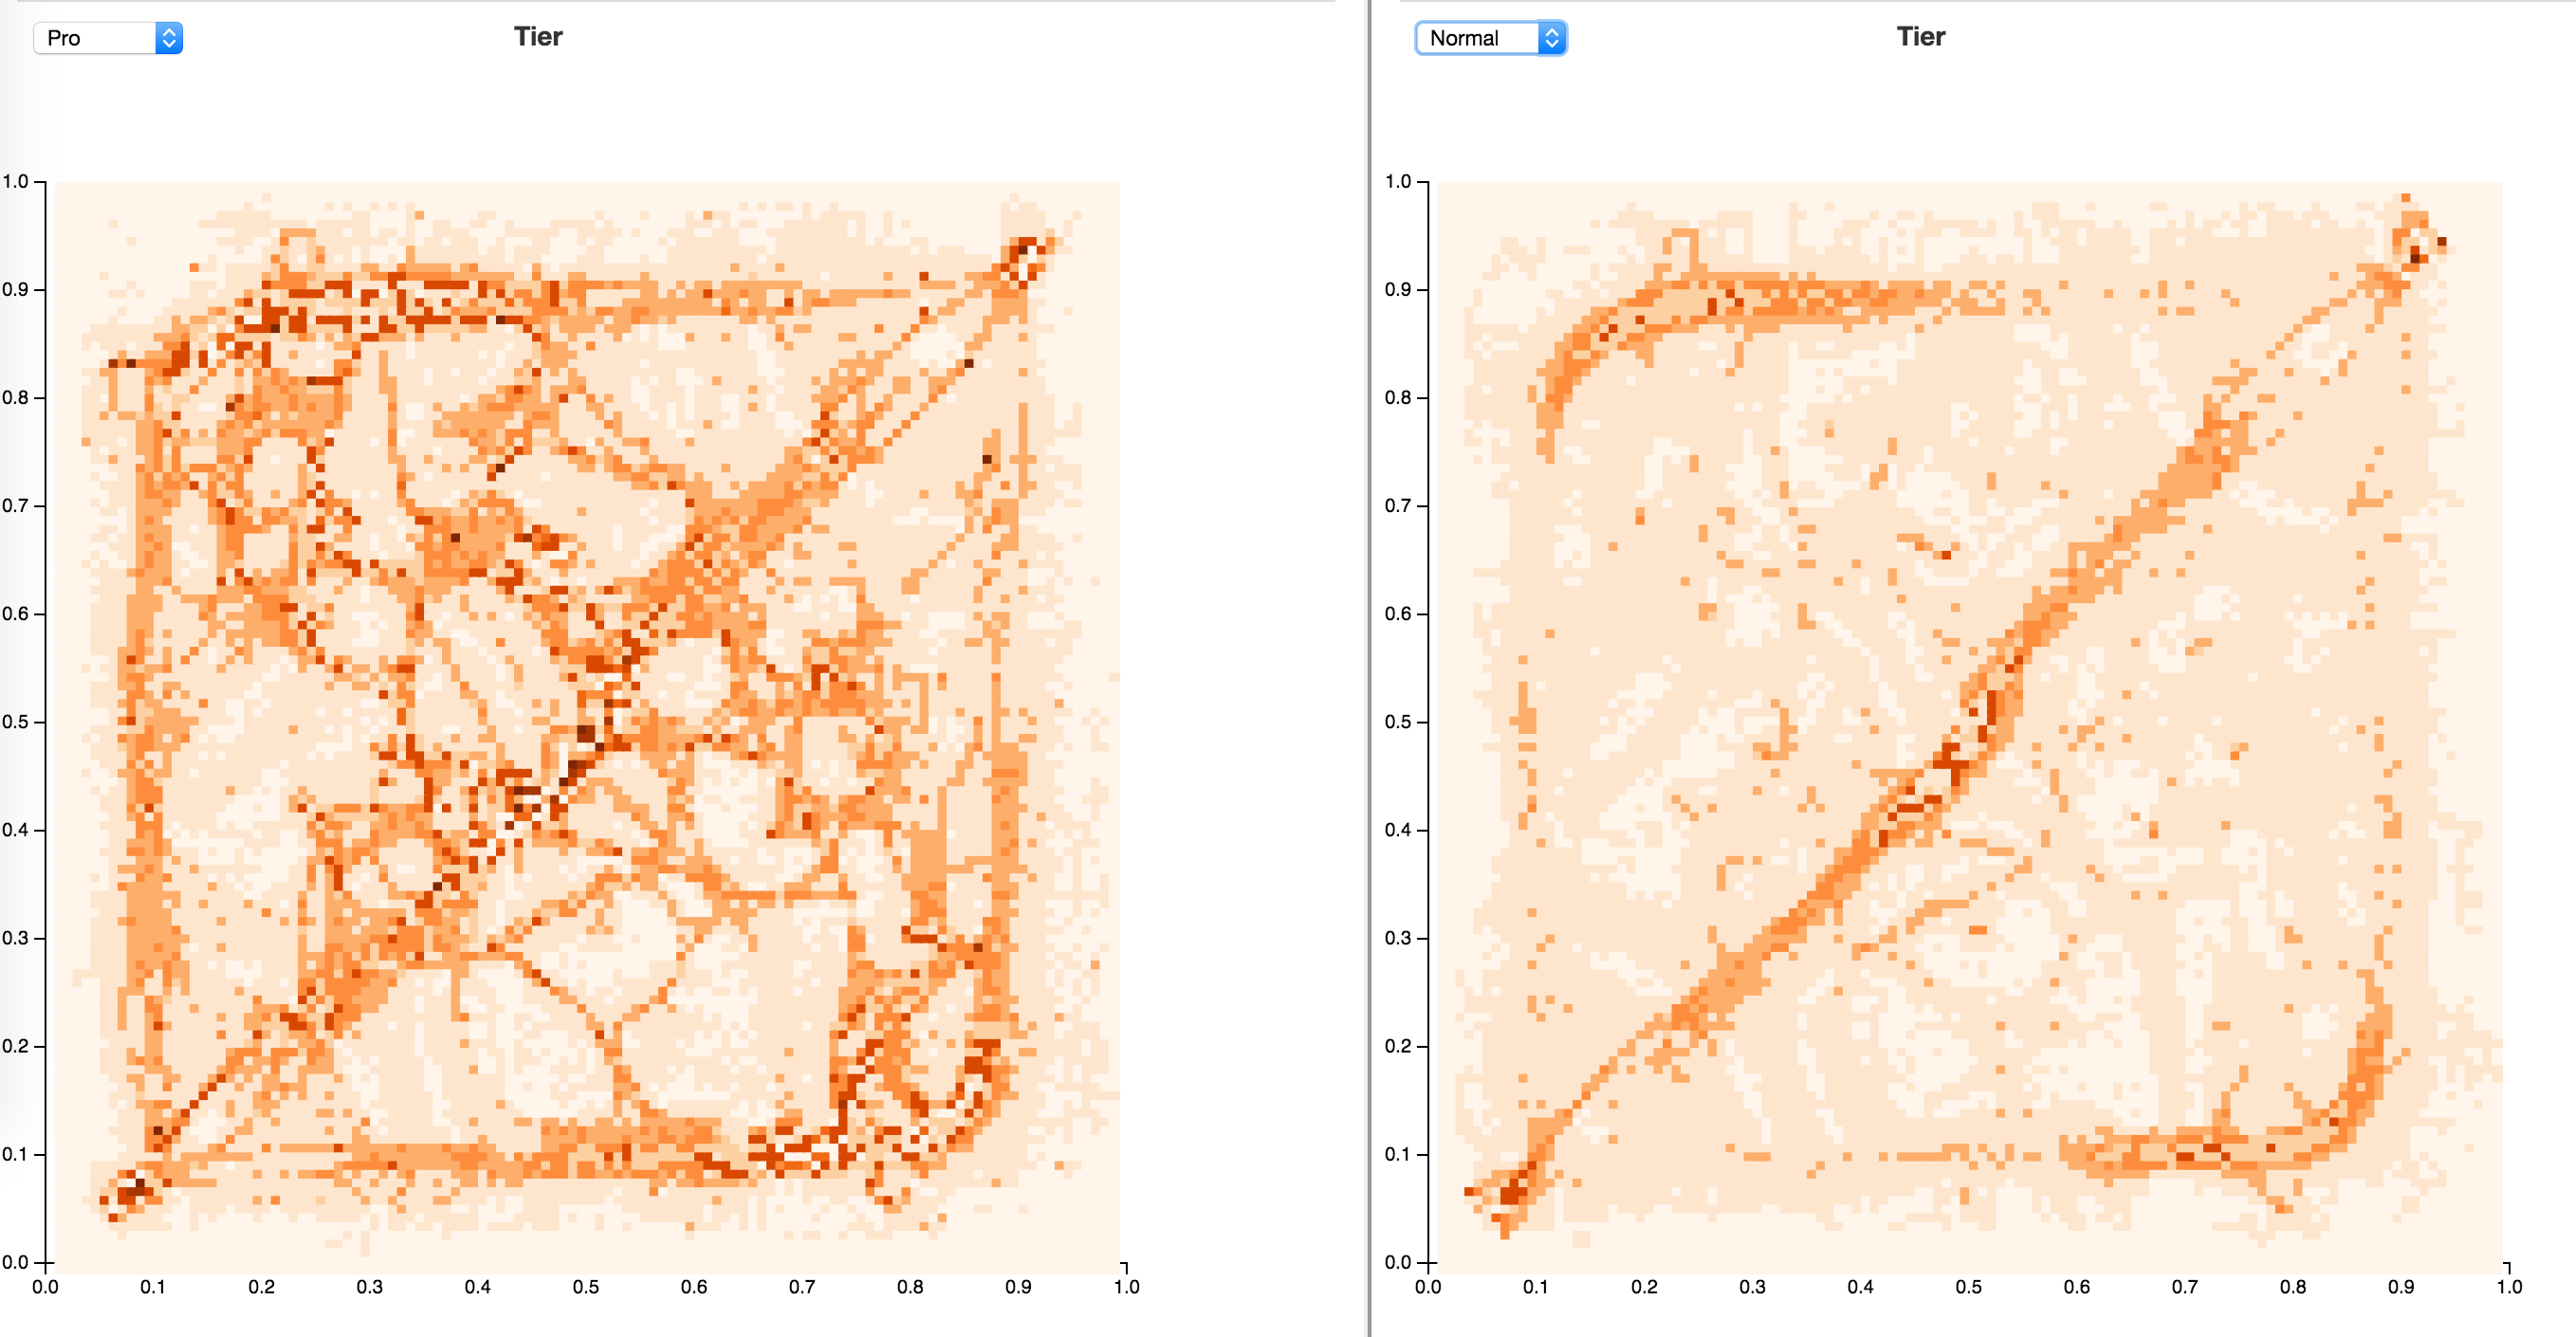
\includegraphics[width=\textwidth]{HM_tiers}

This image compares the heatmaps from low tier and pro tier. We can clearly see how the normal skill tier mostly fights in lanes and rarely fights in the jungle area, while the pro tier spends a lot more time in the jungle.

Here we see the early game, mid game and end game distributions from one match.

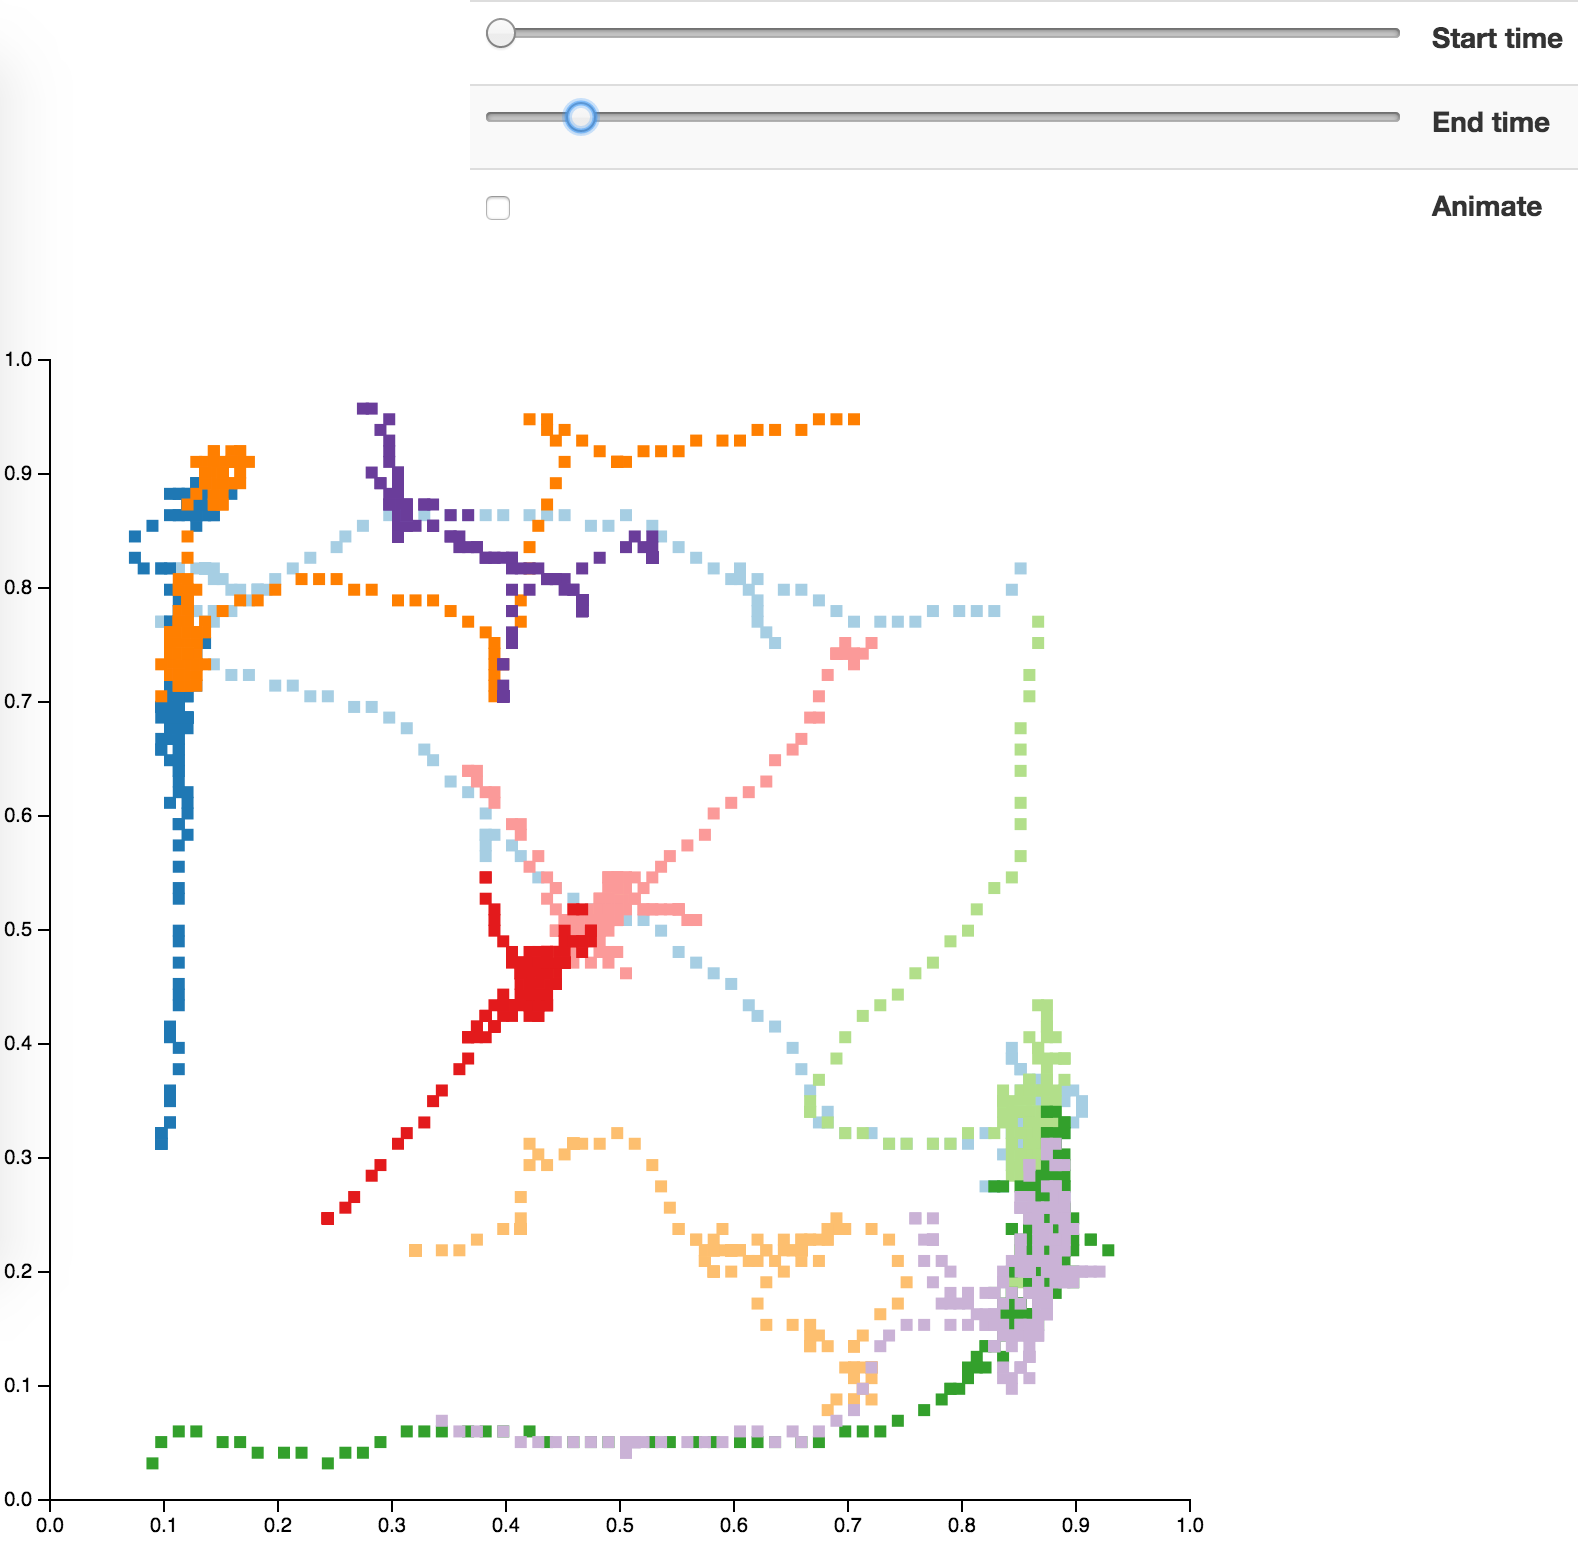
\includegraphics[width=0.7\textwidth]{earlygame}

In the early game we see the players moving into their respective lanes and exchange some blows.

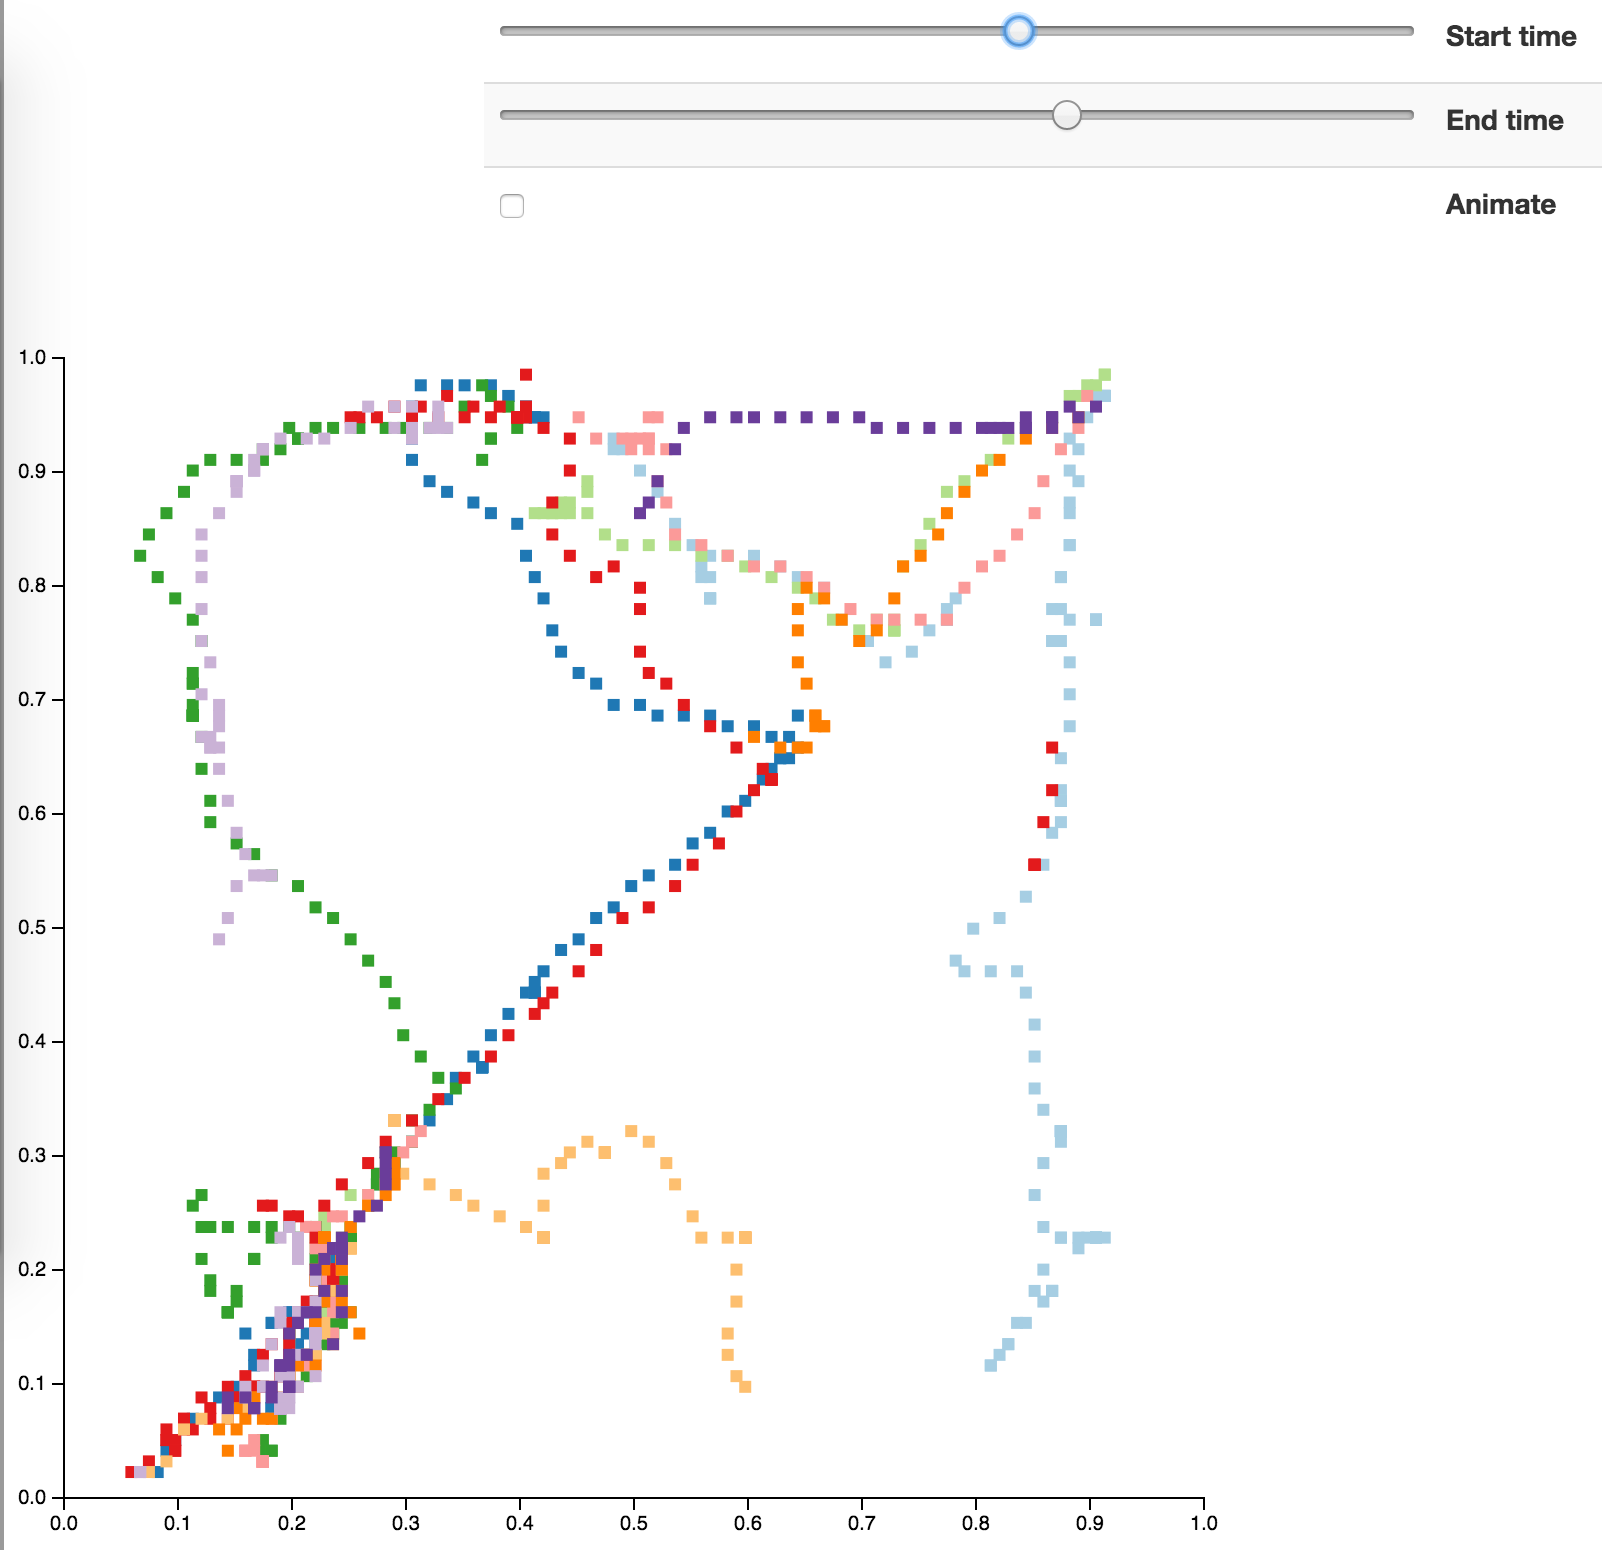
\includegraphics[width=0.7\textwidth]{midgame}

In the late-midgame we see that the game progressed out of their laning phases, and the action is moving towards the bottom team's base. We can see that they most probably lost the middle lane and are behind.

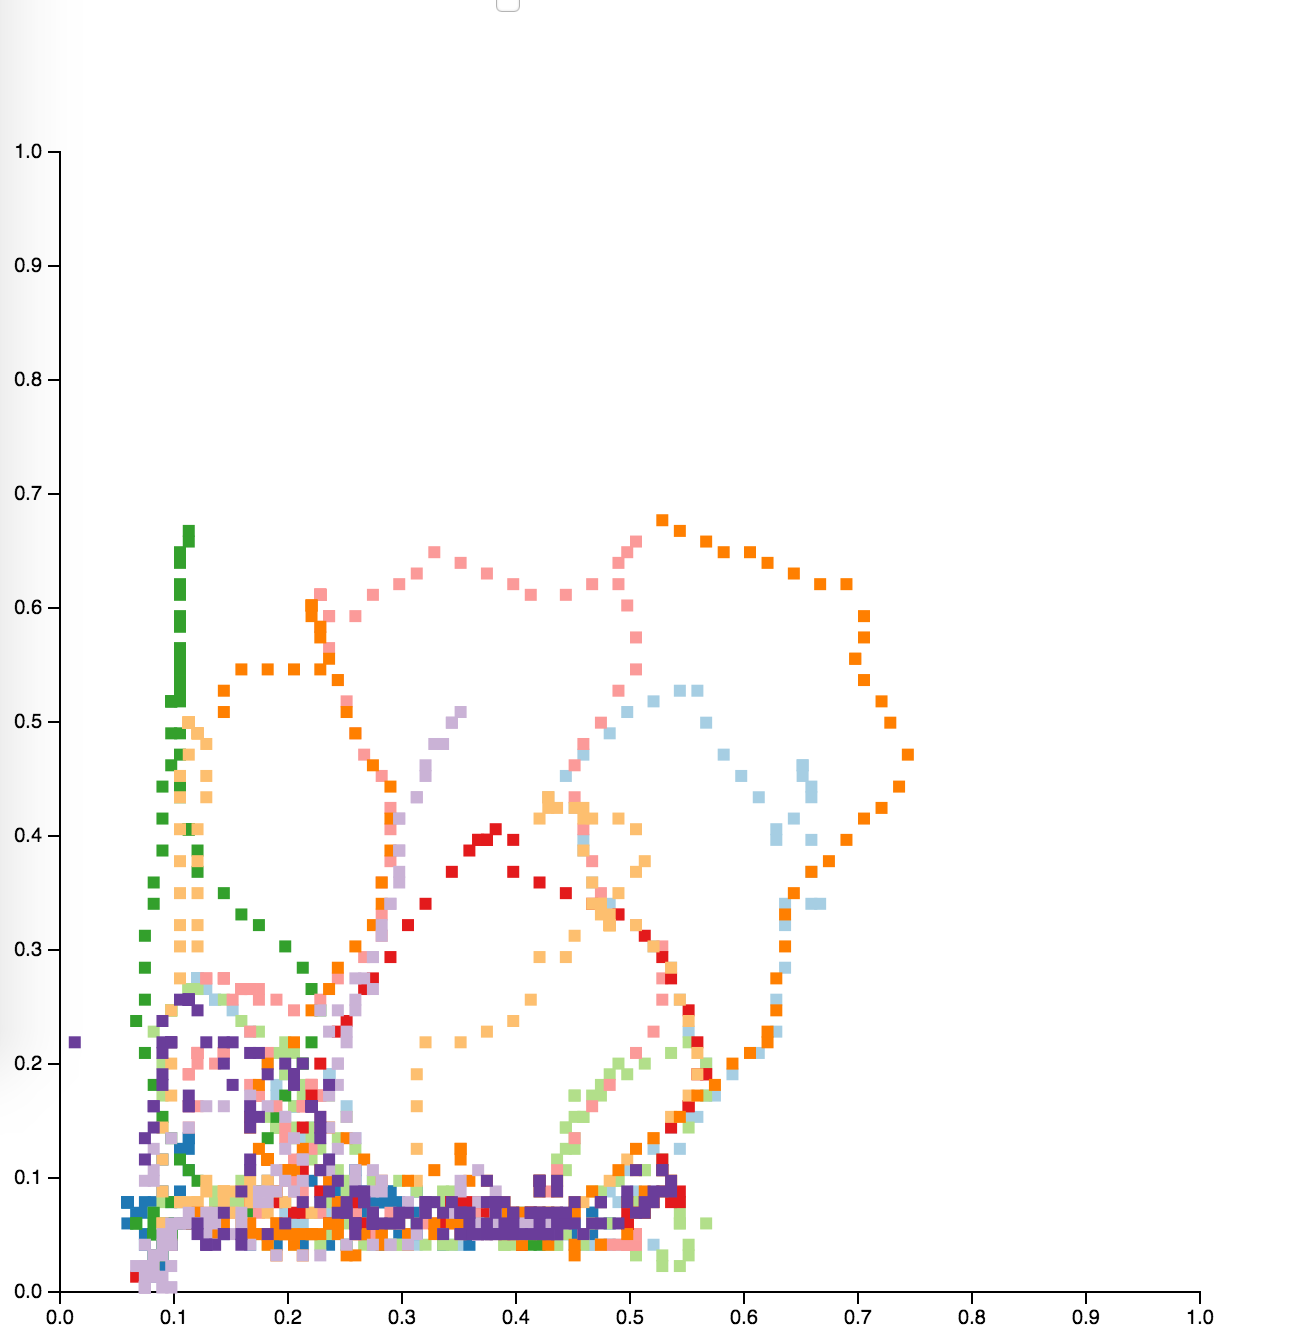
\includegraphics[width=0.7\textwidth]{lategame}

Late game confirms this by exclusively showing heavy fighting in the bottom lane and the bottom team's base. The game ended here, so we can conclude that the top team won.



\end{document}
